%%%%%%%%%%%%%%%%%%%%%%%%%%%%%%%%%%%%%%%%%
% Beamer Presentation
% LaTeX Template
% Version 1.0 (10/11/12)
%
% This template has been downloaded from:
% http://www.LaTeXTemplates.com
%
% License:
% CC BY-NC-SA 3.0 (http://creativecommons.org/licenses/by-nc-sa/3.0/)
%
%%%%%%%%%%%%%%%%%%%%%%%%%%%%%%%%%%%%%%%%%

%----------------------------------------------------------------------------------------
%	PACKAGES AND THEMES
%----------------------------------------------------------------------------------------

\documentclass{beamer}
\usefonttheme[onlymath]{serif}

\usepackage{color}
\usepackage{lmodern}
\usepackage{graphicx}

\mode<presentation> {

% The Beamer class comes with a number of default slide themes
% which change the colors and layouts of slides. Below this is a list
% of all the themes, uncomment each in turn to see what they look like.

%\usetheme{default}
%\usetheme{AnnArbor}
%\usetheme{Antibes}
%\usetheme{Bergen}
%\usetheme{Berkeley}
%\usetheme{Berlin}
\usetheme{Boadilla}
%\usetheme{CambridgeUS}
%\usetheme{Copenhagen}
%\usetheme{Darmstadt}
%\usetheme{Dresden}
%\usetheme{Frankfurt}
%\usetheme{Goettingen}
%\usetheme{Hannover}
%\usetheme{Ilmenau}
%\usetheme{JuanLesPins}
%\usetheme{Luebeck}
% \usetheme{Madrid}
%\usetheme{Malmoe}
%\usetheme{Marburg}
%\usetheme{Montpellier}
%\usetheme{PaloAlto}
%\usetheme{Pittsburgh}
%\usetheme{Rochester}
% \usetheme{Singapore}
%\usetheme{Szeged}
%\usetheme{Warsaw}

% As well as themes, the Beamer class has a number of color themes
% for any slide theme. Uncomment each of these in turn to see how it
% changes the colors of your current slide theme.

%\usecolortheme{albatross}
%\usecolortheme{beaver}
%\usecolortheme{beetle}
%\usecolortheme{crane}
%\usecolortheme{dolphin}
%\usecolortheme{dove}
%\usecolortheme{fly}
%\usecolortheme{lily}
%\usecolortheme{orchid}
%\usecolortheme{rose}
%\usecolortheme{seagull}
% \usecolortheme{seahorse}
%\usecolortheme{whale}
%\usecolortheme{wolverine}

%\setbeamertemplate{footline} % To remove the footer line in all slides uncomment this line
%\setbeamertemplate{footline}[page number] % To replace the footer line in all slides with a simple slide count uncomment this line

%\setbeamertemplate{navigation symbols}{} % To remove the navigation symbols from the bottom of all slides uncomment this line
}

\usepackage{graphicx} % Allows including images
\usepackage{booktabs} % Allows the use of \toprule, \midrule and \bottomrule in tables

%----------------------------------------------------------------------------------------
%	TITLE PAGE
%----------------------------------------------------------------------------------------

\title[Image Processing and Chromatic Derivatives]{Image Processing Applications of Chromatic Derivatives} % The short title appears at the bottom of every slide, the full title is only on the title page

\author{Louis Tiao} % Your name
\institute[UNSW] % Your institution as it will appear on the bottom of every slide, may be shorthand to save space
{
School of Computer Science and Engineering, \\
The University of New South Wales \\ % Your institution for the title page
\medskip
\textit{louis.tiao@student.unsw.edu.au} % Your email address
}
\date{\today} % Date, can be changed to a custom date

\begin{document}

\begin{frame}
\titlepage % Print the title page as the first slide
\end{frame}

\begin{frame}
\frametitle{Overview} % Table of contents slide, comment this block out to remove it
\tableofcontents % Throughout your presentation, if you choose to use \section{} and \subsection{} commands, these will automatically be printed on this slide as an overview of your presentation
\end{frame}

%----------------------------------------------------------------------------------------
%	PRESENTATION SLIDES
%----------------------------------------------------------------------------------------

%------------------------------------------------
\section{Introduction} % Sections can be created in order to organize your presentation into discrete blocks, all sections and subsections are automatically printed in the table of contents as an overview of the talk
%------------------------------------------------

\subsection{Motivation} % A subsection can be created just before a set of slides with a common theme to further break down your presentation into chunks

\begin{frame}
\frametitle{Problems in Image Processing}
\framesubtitle{Border handling for kernel convolutions (linear filters)}

Kernel convolution typically requires pixel values from outside the image boundaries.

\begin{columns}[c] % The "c" option specifies centered vertical alignment while the "t" option is used for top vertical alignment
\column{.45\textwidth} % Left column and width
\begin{enumerate}
	\item Extend
	\item Wrap
	\item Crop
	\item \textbf{Approximate} 
\end{enumerate}
\column{.5\textwidth} % Right column and width
\begin{figure} %[!ht]
\centering
	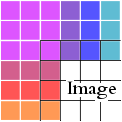
\includegraphics[width=0.3\columnwidth]{../figures/Extend_Edge-Handling}
\caption{Border handling: extend}
\end{figure}
\end{columns}

Make \alert{local} approximations to extend the image in a visually plausible manner.

\end{frame}

%------------------------------------------------

\begin{frame}
\frametitle{Problems in Image Processing}
\framesubtitle{Digital image inpainting}

Reconstructing lost or deteriorated parts of digital images; removing objects from 
digital images and refilling it in a visually plausible manner.

\begin{columns}[c] % The "c" option specifies centered vertical alignment while the "t" option is used for top vertical alignment
\column{.45\textwidth} % Left column and width
Some applications include
\begin{enumerate}
	\item Red-eye/blemish removal
	\item Object/text removal
	\item Art/image restoration
\end{enumerate}
\column{.5\textwidth} % Right column and width
\begin{figure} %[!ht]
\centering
	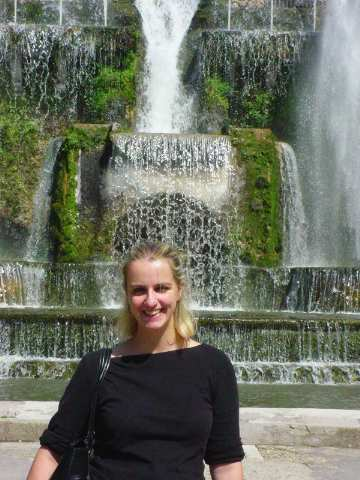
\includegraphics[width=0.45\columnwidth]{../figures/researchmicros-000.jpg}
	\hfill
	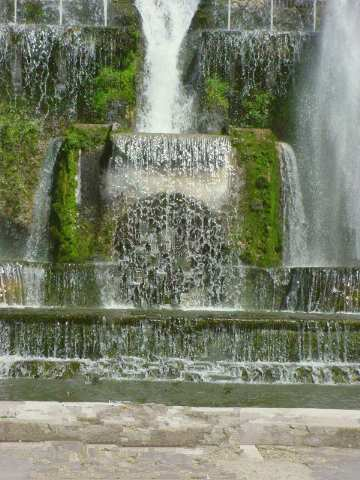
\includegraphics[width=0.45\columnwidth]{../figures/researchmicros-001.jpg}
\caption{Removing large objects from images}
\end{figure}
\end{columns}

\end{frame}

%------------------------------------------------

\begin{frame}
\frametitle{Problems in Image Processing}
\framesubtitle{Digital image inpainting}

Traditionally, inpainting has been done manually by professional conservator-restorers. The methodology is roughly

\begin{columns}[c] % The "c" option specifies centered vertical alignment while the "t" option is used for top vertical alignment
\column{.55\textwidth} % Left column and width
\begin{enumerate}
	\item Global image determines how to fill gap; restore the unity of the work.
	\item Structural details surrounding the gap (\alert{local} info.) must be
	 pronlonged into the gap. E.g. countours lines.
	\item Similar for details in colour and texture.
\end{enumerate}
Current computerized/digital methods try to emulate this process.

\column{.45\textwidth} % Right column and width
\begin{figure} %[!ht]
\centering
	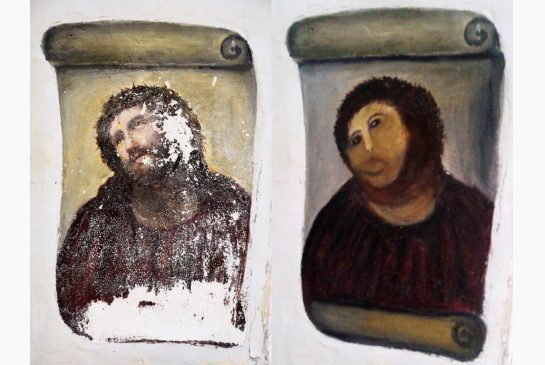
\includegraphics[width=\columnwidth]{../figures/fresco.jpg}
\caption{\textit{Ecce `Mono'}: A failed restoration}
\end{figure}
\end{columns}

\end{frame}

%------------------------------------------------

\begin{frame}
\frametitle{A Signal Processing Problem}

In other words...

\begin{itemize}
	\item Forecast/predict the missing values and extend/fill the image with our estimation.
	\item Very unusual signal processing problem - we are interested extremely local signal behaviour. 
\end{itemize}

\end{frame}



\begin{frame}
\frametitle{Fourier series}
\begin{columns}[c]
\column{.6\textwidth}
\begin{itemize}
	\item Let $f(t)$ be a signal in the time domain with period $2T$. Its 
		\textit{Fourier series} expansion is given by

		\begin{align}
			f(t)	&= \sum_{n=-\infty}^{\infty} c_n e^{i \frac{\pi n}{T} t} \\
			c_n		&= \frac{1}{2T} \int_{-T}^{T} f(t) e^{-i \frac{\pi n}{T} t} dt
		\end{align}
	\item \textbf{Global}, approximates local behaviour poorly
	\item Indispensable to digital signal processing (DSP)
	% TODO: Insert complex exponential identities (?)
\end{itemize}
\column{.4\textwidth}
\begin{figure} %[!ht]
\centering
	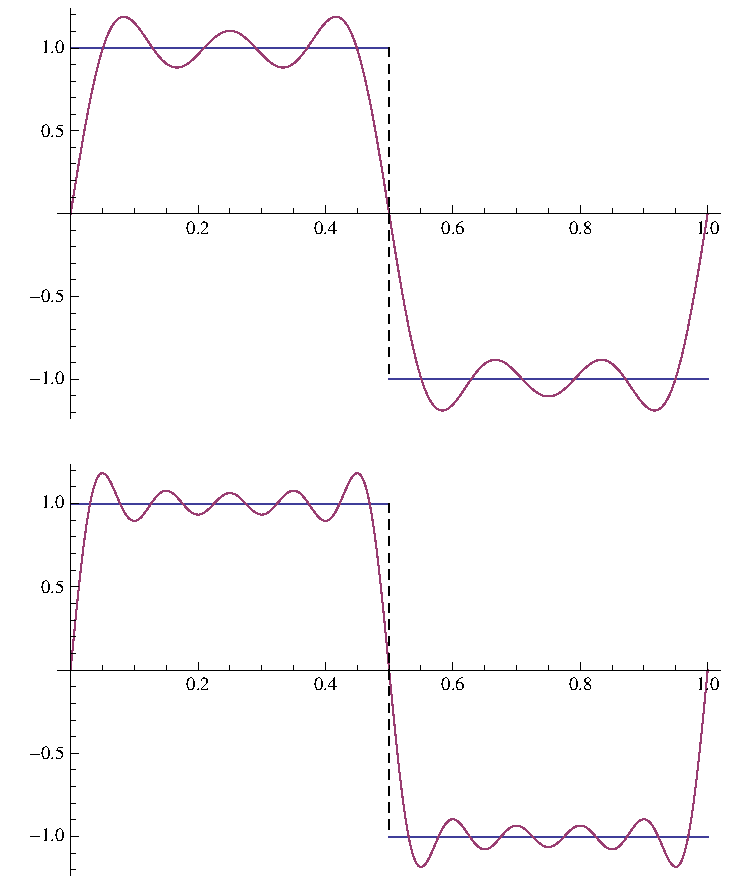
\includegraphics[width=\columnwidth]{../figures/fourier}
\caption{Truncated Fourier expansion of orders 11 (top) and 21 (bottom)}
\end{figure}
\end{columns}
\end{frame}

%------------------------------------------------

\begin{frame}
\frametitle{Whittaker-Shannon interpolation formula}
\begin{itemize}
	\item If $f \in \mathbf{BL}(\pi)$, i.e. $f \in L^2$ and $\hat{f}(\omega)$ 
		supported on $[-\pi, \pi]$, we can derive the \textit{Whittaker-Shannon
		interpolation formula}
		\begin{align}
		f(t)	&= \sum_{n=-\infty}^{\infty} f(n) \mathrm{sinc}{\pi(t-n)} \left (
				= \sum_{n=-\infty}^{\infty} f(n) \frac{\sin{\pi(t-n)}}{\pi(t-n)}
				\right )
		\end{align}
	\item \textbf{Global}, approximates local behaviour poorly
	\item Indispensable to digital signal processing (DSP)
\end{itemize}
\end{frame}

%------------------------------------------------

\begin{frame}
\frametitle{Taylor series}
\begin{columns}[c]
\column{.6\textwidth}
\begin{itemize}
	\item The \textit{Taylor series} expansion of $f(t)$ (about point $t=t_0$) is given by

	\begin{align*}
		f(t)	&= \sum_{n=0}^{\infty} c_n \frac{(t-t_0)^n}{n!} \\
		c_n		&= \mathcal{D}^n[f](t_0) = \mathcal{D}_t^n f(t) |_{t=t_0} \\
				&= \frac{d^n}{dt^n} f(t) |_{t=t_0} = f^{(n)}(t_0)
	\end{align*}
	\item \textbf{Local}
	\item Of limited use to DSP. \alert{Why?}
\end{itemize}
\column{.4\textwidth}
\begin{figure} %[!ht]
\centering
	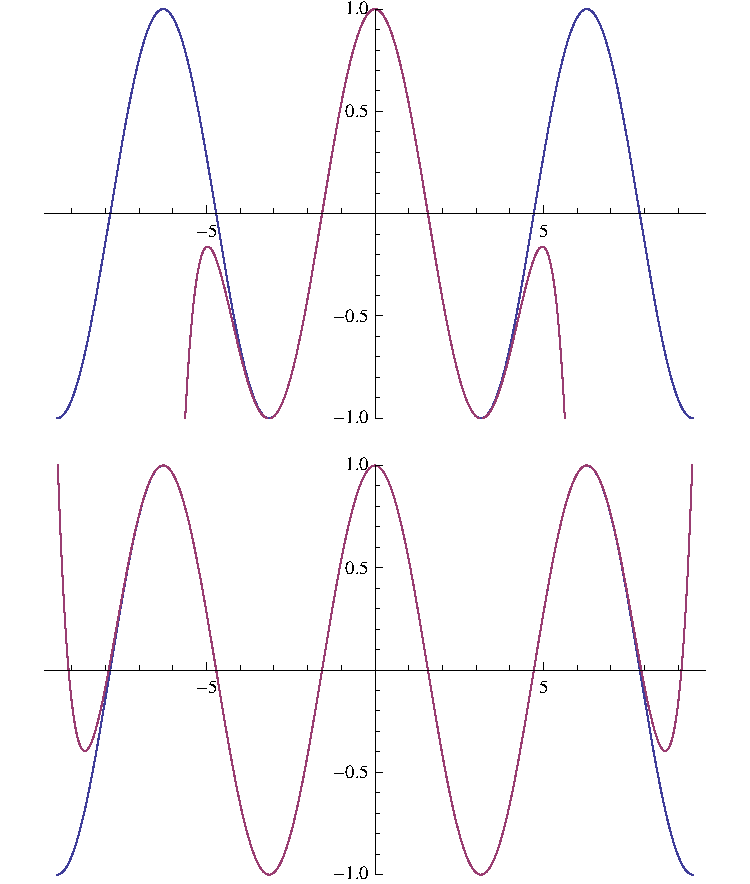
\includegraphics[width=\columnwidth]{../figures/taylor}
\caption{Truncated Taylor expansion of orders 11 (top) and 21 (bottom)}
\end{figure}
\end{columns}

\end{frame}

%------------------------------------------------

\begin{frame}
\frametitle{Shortcomings of the Taylor series expansion}
\begin{itemize}
	\item Numerical evaluation of high order derivatives is \alert{very noise
		sensitive and infeasible.}
	\item Truncations of the Whittaker-Shannon interpolation of all 
		$f \in \mathbf{BL}(\pi)$ has the following properties
		\begin{itemize}
			\item belongs to $\mathbf{BL}(\pi)$
			\item converges to $f$ uniformly and in $L^2$
			\item if $A$ is a (continuous, linear, time-invariant) filter, then
				\begin{equation} \label{eqn:filter_prop}
					A[f](t) = \sum_{n=-\infty}^{\infty} f(n) A[\mathrm{sinc}](t-n)
				\end{equation}
		\end{itemize}
		In stark contrast, \alert{none of these important properties hold} for
		truncations of a Taylor series expansion of any $f \in \mathbf{BL}(\pi)$.
		% TODO: Obliterates spectrum (?)
\end{itemize}
\end{frame}

%------------------------------------------------

\begin{frame}
\frametitle{Comparison: Taylor/Fourier series}
\begin{table}
\begin{tabular}{c c c}
\toprule
Expansion & \textbf{Fourier} & \textbf{Taylor}\\
\midrule
Physical Interpret. & Frequency component & Gradient component \\
Approx. & Global & \textcolor{blue}{Local} \\
Basis			& $e^{i \frac{\pi n}{T} t}$ & $\frac{(t-t_0)^n}{n!}$ \\
Basis type 		 & Sinusoids & Monomials \\
Basis Orthog.& \textcolor{blue}{Yes} & \alert{No} \\
Coefficient & $\frac{1}{2L} \int_{-L}^{L} f(t) e^{-i \frac{\pi n}{L} t} dt$ & $\mathcal{D}^n[f](t_0)$ \\
Coef. type  & Integral & \alert{Derivative} \\
\bottomrule
\end{tabular}
\end{table}

\begin{itemize}
	\item Can we find a better base for the space of linear differential operators?
	\item Furthermore, an \alert{orthogonal basis}?
\end{itemize}
\end{frame}

%------------------------------------------------
\section{Background}
%------------------------------------------------

\subsection{Chromatic Derivatives}

\begin{frame}
\frametitle{Overview of Chromatic Derivatives}
\begin{itemize}
	\item Dr. Aleks Ignjatovic introduced \textit{Chromatic derivatives} 
	(c.f. \cite{Ignjatovic2009} for recent publication)
	\item \textbf{Key Concept:} Instead of $n$th-order derivatives, consider linear 
	combinations of lower order derivatives
	\begin{equation*}
		\mathcal{D}_t^n \leftarrow P_n(\mathcal{D}_t) = \sum_{k=0}^{n} c_k \mathcal{D}_t^k
	\end{equation*}
	where $P_n$ is an \alert{orthogonal polynomial}. E.g.
	\begin{itemize}
		\item Legendre polynomyials
		\item Chebyshev polynomials
		\item Hermite polynomials
		\item Et cetera.
	\end{itemize}
\end{itemize}
\end{frame}

%------------------------------------------------

\begin{frame}
\frametitle{Chromatic Derivatives}
\framesubtitle{Associated with Legendre Polynomials}
\begin{itemize}
\item Solutions to Legendre's differential equation
\begin{equation*}
\frac{d}{dx}\left[(1-x^2)\frac{d}{dx}P_n(x)\right]+n(n+1)P_n(x)=0
\end{equation*}
\item Defined by the recurrence
\begin{align*}
P_0(x) &= 1, P_1(x) = x \\
P_{n+1}(x) &= \frac{2n+1}{n+1}xP_n(x) - \frac{n}{n+1}P_{n-1}(x)
\end{align*}
\item \alert{Orthogonal} and \alert{complete} over $[-1, 1]$
\begin{equation*}
\int_{-1}^{1} P_n(x)P_m(x) dx = \frac{2}{2n+1} \delta_{mn}
\end{equation*}
where $\delta_{mn}$ is the Kronecker delta.
\end{itemize}
\end{frame}

%------------------------------------------------


\begin{frame}
\frametitle{Chromatic Derivatives}
\framesubtitle{Associated with Legendre Polynomials}
\begin{columns}[c]
\column{.55\textwidth}
\begin{itemize}
	\item Rescale and normalize
		over $[-\pi, \pi]$
	\begin{equation*}
		P_n^L(x) = \sqrt{2n+1}P_n\left(\frac{x}{\pi}\right)
	\end{equation*}
	\item \alert{Orthogonal} and \alert{complete} over $[-\pi, \pi]$
	\begin{equation*}
		\frac{1}{2\pi} \int_{-\pi}^{\pi} P_n^L(x) P_m^L(x) dx = \delta_{mn}
	\end{equation*}
\end{itemize}
\column{.35\textwidth}
\begin{figure} %[!ht]
\centering
	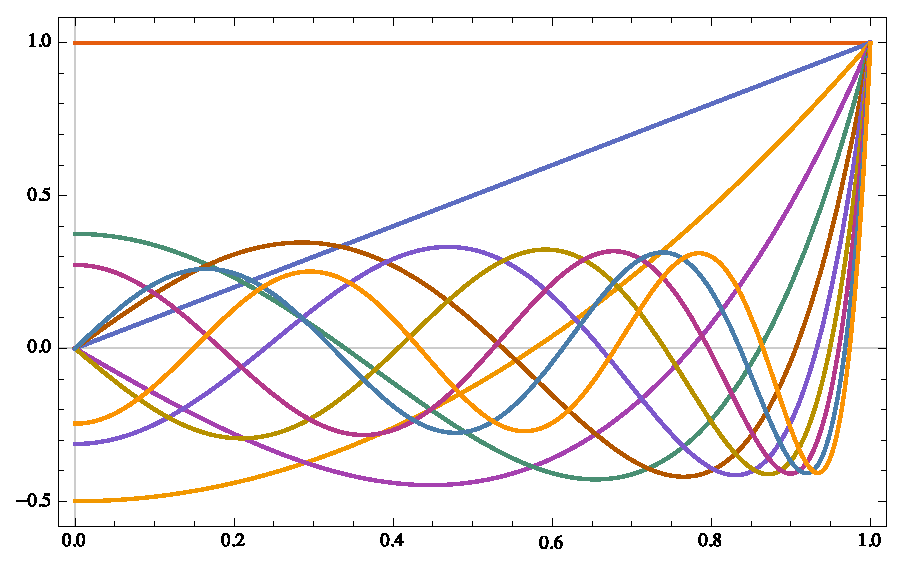
\includegraphics[width=\columnwidth]{../figures/legendre}
\caption{First 10 Legendre polynomials}
\end{figure}
\end{columns}
\pause
\begin{example}[First few Legendre polynomials]
\begin{align*}
& P_0(x) = 1, & P_2(x) = \frac{1}{2}(3x^2-1), \\
& P_1(x) = x, 
& P_3(x) = \frac{1}{2}(5x^3-3x)
\end{align*}
\end{example}
\end{frame}

%------------------------------------------------

\begin{frame}
\frametitle{Chromatic Derivatives}
The chromatic derivatives associated with Legendre polynomials of order $n$ 
with respect to $t$ is defined as
\begin{equation}
	\mathcal{K}_t^n = (-i)^n P_n^L(i\mathcal{D}_t)
\end{equation}
where $\mathcal{D}_t$ is the differential operator with respect to $t$ and
$P_n^L$ are the normalized and scaled Legendre polynomials.
\pause
\begin{example}[Derivative vs. chromatic derivative]
\begin{table}
\begin{tabular}{l l}
 & Operator \\
\midrule
Derivative & $\mathcal{D}_t^3$ \\
Chromatic Derivative & $\mathcal{K}_t^3 = \frac{\sqrt{7}}{2\pi} \left ( \frac{5}{\pi^2} \mathcal{D}_t^3 + 3 \mathcal{D}_t \right )$ \\
\bottomrule
\end{tabular}
\caption{A 3rd order derivative and 3rd order chromatic derivative}
\end{table}
\end{example}
\end{frame}

%------------------------------------------------

\begin{frame}
\frametitle{Chromatic Derivatives}
\begin{itemize}
	\item We can easily verify that
		\begin{equation*}
			\mathcal{K}_t^n[e^{i\omega t}] = i^n P_n^L(\omega) e^{i\omega t}
		\end{equation*}
	\item So for $f \in \mathbf{BL}(\pi)$, we have
		\begin{equation}
			\mathcal{K}^n[f](t) = \frac{1}{2\pi} \int_{-\pi}^{\pi} i^n P_n^L(\omega) \hat{f}(\omega) e^{i\omega t} d\omega
		\end{equation}
		% TODO: Why
\end{itemize}
\end{frame}

%------------------------------------------------

\begin{frame}
\frametitle{Chromatic Derivatives}
\begin{itemize}
	\item The Fourier series expansion of $\hat{f}(\omega)$ is given by
		 \begin{align*}
			\hat{f}(\omega)	&= \sum_{n=0}^{\infty} c_n (-i)^n P_n^L(\omega) \\
			c_n							&= \frac{1}{2\pi} \int_{-\pi}^{\pi} i^n P_n^L(\omega) \hat{f}(\omega) d\omega
										= \mathcal{K}^n[f](0)
		\end{align*}
	\item By taking the inverse Fourier transform on $\omega$, we get the \textit{chromatic expansion}
		\begin{equation*}
			f(t)	= \sum_{n=0}^{\infty} (-1)^n  \mathcal{K}^n[f](0) \mathcal{K}^n[\mathrm{sinc}](t)
					= \sum_{n=0}^{\infty} \mathcal{K}^n[f](0) \sqrt{2n+1} j_n(\pi t)
		\end{equation*}
		where $j_n(t) = \sqrt{\frac{\pi}{2x}}J_{n+1/2}(x)$ is the spherical Bessel function of the first kind.
\end{itemize}
\end{frame}

%------------------------------------------------

\begin{frame}
\frametitle{Putting it all together}

\begin{block}{Taylor series expansion}
\begin{equation*}
	f(t) = \sum_{n=0}^{\infty} \mathcal{D}^n[f](0) \frac{t^n}{n!}
\end{equation*}
\end{block}

\begin{block}{Chromatic series expansion}
\begin{equation*}
	f(t) = \sum_{n=0}^{\infty} \mathcal{K}^n[f](0) \sqrt{2n+1} j_n(\pi t)
\end{equation*}
\end{block}

\begin{block}{Shannon-Whittaker interopolation}
\begin{equation*}
	f(t) = \sum_{n=-\infty}^{\infty} f(n) \mathrm{sinc}{\pi(t-n)}
\end{equation*}
\end{block}

\end{frame}

%------------------------------------------------

\begin{frame}
\frametitle{Comparison: approximation}

\begin{figure} %[!ht]
\centering
	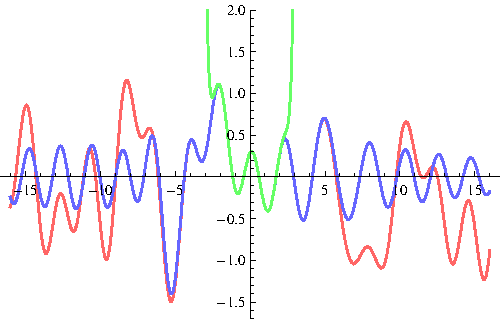
\includegraphics[width=0.8\columnwidth]{../figures/approx}
\caption{\textcolor{red}{red:} original signal; 
\textcolor{blue}{red:} chromatic approx. of order 15;
\textcolor{green}{green:} Taylor approx. of order 15}
\end{figure}

\end{frame}

%------------------------------------------------

\begin{frame}
\frametitle{Comparison of the Expansions}

\begin{table}
\begin{tabular}{c c c p{2cm}}
\toprule
\textbf{Expansion} & Taylor & Chromatic & Whittaker-Shannon\\
\midrule
Local approx. & Best & Good & Poor \\
Global approx. & Poor & Good & Best \\
Uniform convergence & No & Yes & Yes \\
Band-limited & No & Yes & Yes \\
Noise tolerance & Low & High & - \\
Filter prop. (\ref{eqn:filter_prop}) & No & Yes & Yes \\
\bottomrule
\end{tabular}
\caption{Summary of the various expansions}
\end{table}

\textbf{Upshot:} The chromatic expansions possesses the same properties 
that make the Whittaker-Shannon interpolation essential to signal processing.

% todo uniform convergence in R

\end{frame}

%------------------------------------------------

\begin{frame}
\frametitle{Back to Image Processing...}

\begin{columns}[c]
\column{.45\textwidth}
\begin{itemize}
	\item Regularization to prevent overfitting
	\item Linear programming to fit subject to constraints - 
		continuity across gaps
\end{itemize}
\column{.5\textwidth}
\begin{figure} %[!ht]
\centering
	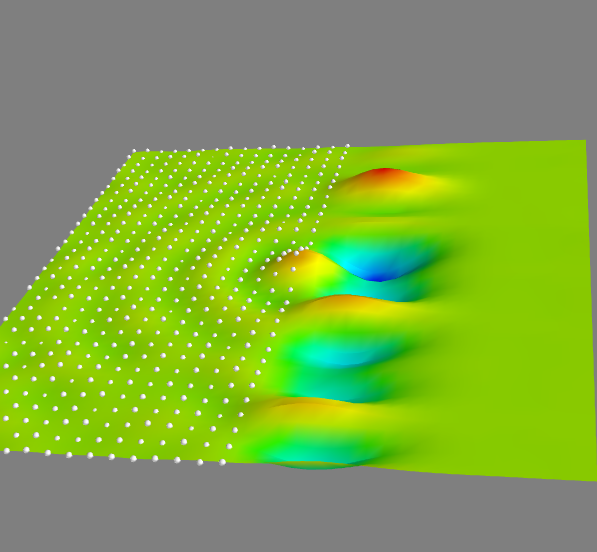
\includegraphics[width=\columnwidth]{../figures/31x16bump.png}
\caption{Chromatic expansion of a signal in the spatial domain; 
dots are samples and surface is the expansion}
\end{figure}
\end{columns}

\end{frame}

% ------------------------------------------------

\subsection{Previous work}

\begin{frame}
\frametitle{Digital Image Inpainting}
\framesubtitle{Conventional methods in previous work}

Previous work in the literature dominated by these methods

\begin{itemize}
	\item structure inpainting\cite{Bertalmio2000}

	\textit{focus on consistency of the geometric structure}

	\item texture inpainting

	\textit{repetitive two-dimensional synthesized texture patterns}

	\item combination of above\cite{Criminisi2004}
\end{itemize}
        
Must consider these as part of our evaluation framework. \\~

\textit{But focus will be investigating novel techniques involving 
chromatic approximations.}

\end{frame}

% ------------------------------------------------

\section{Proposal}

\subsection{Project Plan}
% ------------------------------------------------

\begin{frame}
\frametitle{Project Plan}

\begin{enumerate}
	\item Complete literature review/background readings
	\begin{itemize}
		\item Familiarization with existing inpainting methods
			and general image processing techniques
		\item Papers on chromatic derivatives and preliminaries
	\end{itemize}
	\item Establish evaluation framework
	\begin{itemize}
		\item Reproduce existing inpainting methods to serve as baseline  
	\end{itemize}
	\item Devise methods for inpainting based on chromatic expansions
	\begin{itemize}
		\item Regularized least squares 
		\item Linear programming 
	\end{itemize}
	\item Implement
	\item Experiment/Benchmark
	\item Analyse results, identify potential improvements and repeat from 4
\end{enumerate}


\end{frame}
% ------------------------------------------------

\section{Conclusion}
% ------------------------------------------------

\begin{frame}
\frametitle{Summary}

In this talk, we

\begin{itemize}
	\item saw some interesting problems in image processing - image inpainting 
		- which require local signal behaviour
	\item motivated chromatic derivatives by examining the shortcomings 
		of Taylor series expansions
	\item examined chromatic derivatives in some detail
	\item discussed how to use it to tackle related image processing problems
		and a plan to carry out this project
\end{itemize}

\pause

\begin{center}
\Large Thank you
\end{center}

\end{frame}
% ------------------------------------------------

\subsection{Bibliography}
% ------------------------------------------------

\begin{frame}[allowframebreaks]
	\frametitle{References}
	Portions of this talk are derived from previous talks given by \cite{Ignjatovic2011,Liu2011}.

	\bibliographystyle{plain}
	\bibliography{../bibliography}
\end{frame}

%----------------------------------------------------------------------------------------

\end{document} 